\subsection{Bifurcação}

A família quadrática exibe outro fenômeno que ocorre em sistemas dinâmicos: a bifurcação.
Através desse fenômeno, vamos explicar gráfica e intuitiva como a dinâmica de $h$, que é simples para $\mu$ pequeno, se torna caótica para $\mu$ suficientemente grande.

Seja $f_\lambda$ uma família parametrizada de funções no parâmetro $\lambda$ de modo que a função
$$G(x, \lambda) = f_\lambda(x),$$
definida num aberto de $\RR^2$, seja de classe $\class^\infty$ nas variáveis $x$ e $\lambda$.
Dizemos que $f_\lambda$ sofre uma bifurcação em $\lambda_0$ se existe $\varepsilon > 0$ com a seguinte propriedade: se $\lambda_1 \in (\lambda_0 - \varepsilon, \lambda_0)$ e $\lambda_2 \in (\lambda_0, \lambda_0 + \varepsilon)$, então $f_{\lambda_1}$ e $f_{\lambda_2}$ não são topologicamente conjugadas.
Por exemplo, uma bifurcação ocorre quando há alteração na estrutura dos pontos periódicos.

\begin{example}
\begin{enumerate}[label=\alph*)]\item[]
\item 
A família $E_\lambda$ de funções dadas por $E_\lambda(x) = e^{x + \lambda}$ sofre uma bifurcação em $\lambda_0 = -1$.

Conforme o parâmetro cresce, os dois pontos fixos vão se aproximando até se tornarem um único ponto fixo que, após isso, desaparece. Uma bifurcação com essas características é chamada de bifurcação tangente.
\begin{center}
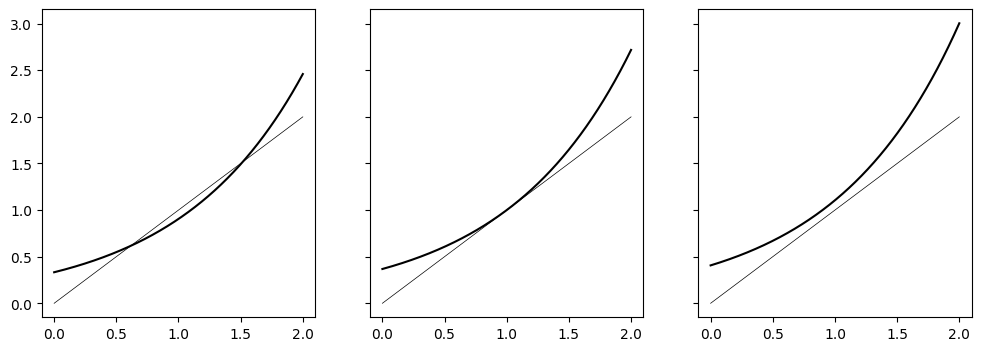
\includegraphics[scale=0.3]{images/e_lambda.png}
\end{center}

\item A família quadrática sofre uma bifurcação em $\mu_0 = 3$.

Conforme o parâmetro cresce, o ponto fixo, que inicialmente é atrator, se torna repulsor e, além disso, nasce uma órbita periódica de período $2$ numa vizinhança do ponto fixo. Uma bifurcação com essas características é chamada de bifurcação com duplicação de período.
\begin{center}
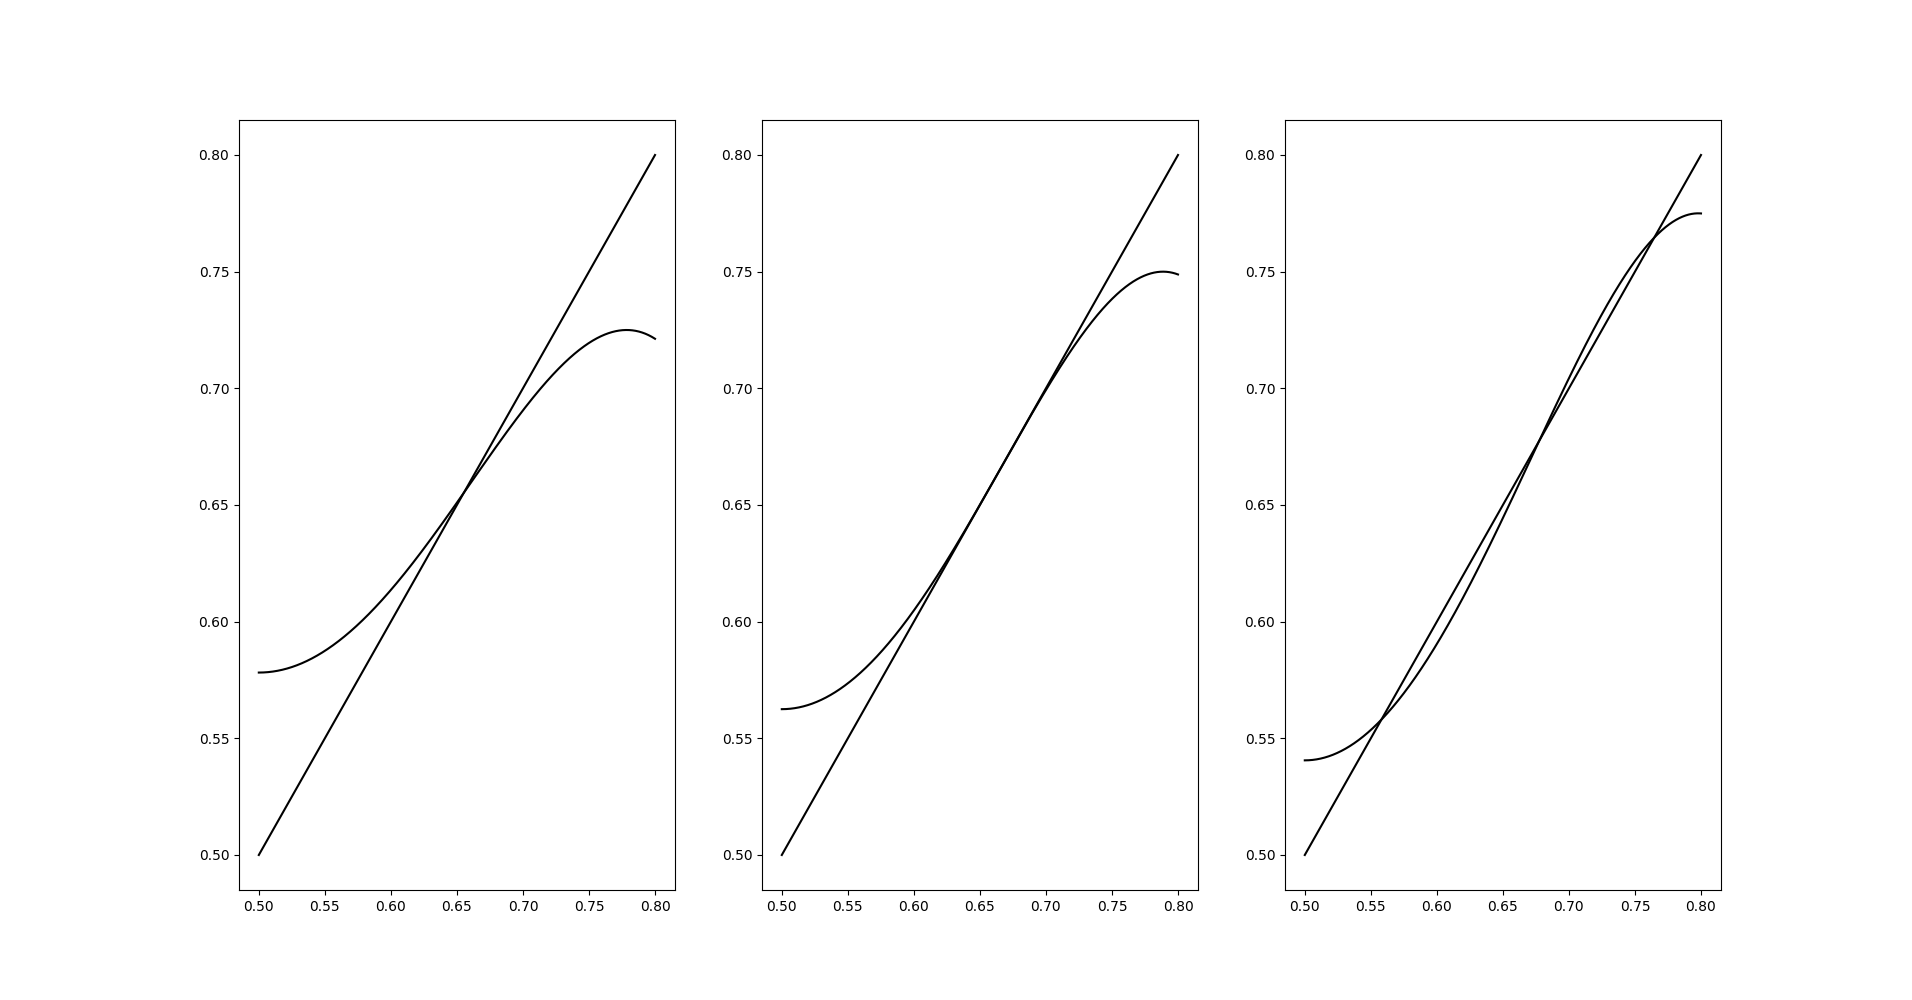
\includegraphics[scale=0.3]{images/h_mu^2.png}
\end{center}
\end{enumerate}
\end{example}

Observe, nos exemplos, que as bifurcações ocorreram quando a derivada em módulo no ponto fixo se tornou igual à $1$. O teorema a seguir nos mostra que isso não é coincidência.

\begin{theorem}\label{theorem1}
Seja $f_\lambda$ uma família parametrizada de funções.
Suponha que
\begin{enumerate}
\item $f_{\lambda_0}(x_0) = x_0$,
\item $f'_{\lambda_0}(x_0) \neq 1$. 
\end{enumerate}
Então existem vizinhanças $I$ e $J$ de $\lambda_0$ e $x_0$, respectivamente, e uma função $p: I \to J$ de classe $\class^\infty$ tais que
\begin{enumerate}
\item $p(\lambda_0) = x_0$, 
\item $f_\lambda(p(\lambda)) = p(\lambda)$ para todo $\lambda \in I$.
\end{enumerate}
Além disso, $f_\lambda$ não possui outros pontos fixos em $J$.
\end{theorem}

\begin{proof}
Basta aplicar o Teorema da Função Implícita para a função $G(x, \lambda) = f_\lambda(x) - x$ no ponto $(x_0, \lambda_0)$.
\end{proof}

Vamos estudar com mais detalhes a bifurcação com duplicação de período que ocorre na família quadrática.
Inicialmente, observe que se $\mu > 2$, então existe $p_\mu' < p_\mu$ tal que $h(p_\mu') = p_\mu$.
Observe o gráfico de $h^2$, juntamente com um quadrado de vértices $(p_\mu', p_\mu)$, $(p_\mu, p_\mu)$, $(p_\mu, p_\mu')$ e $(p_\mu', p_\mu')$, para alguns valores de $\mu$.
\begin{center}
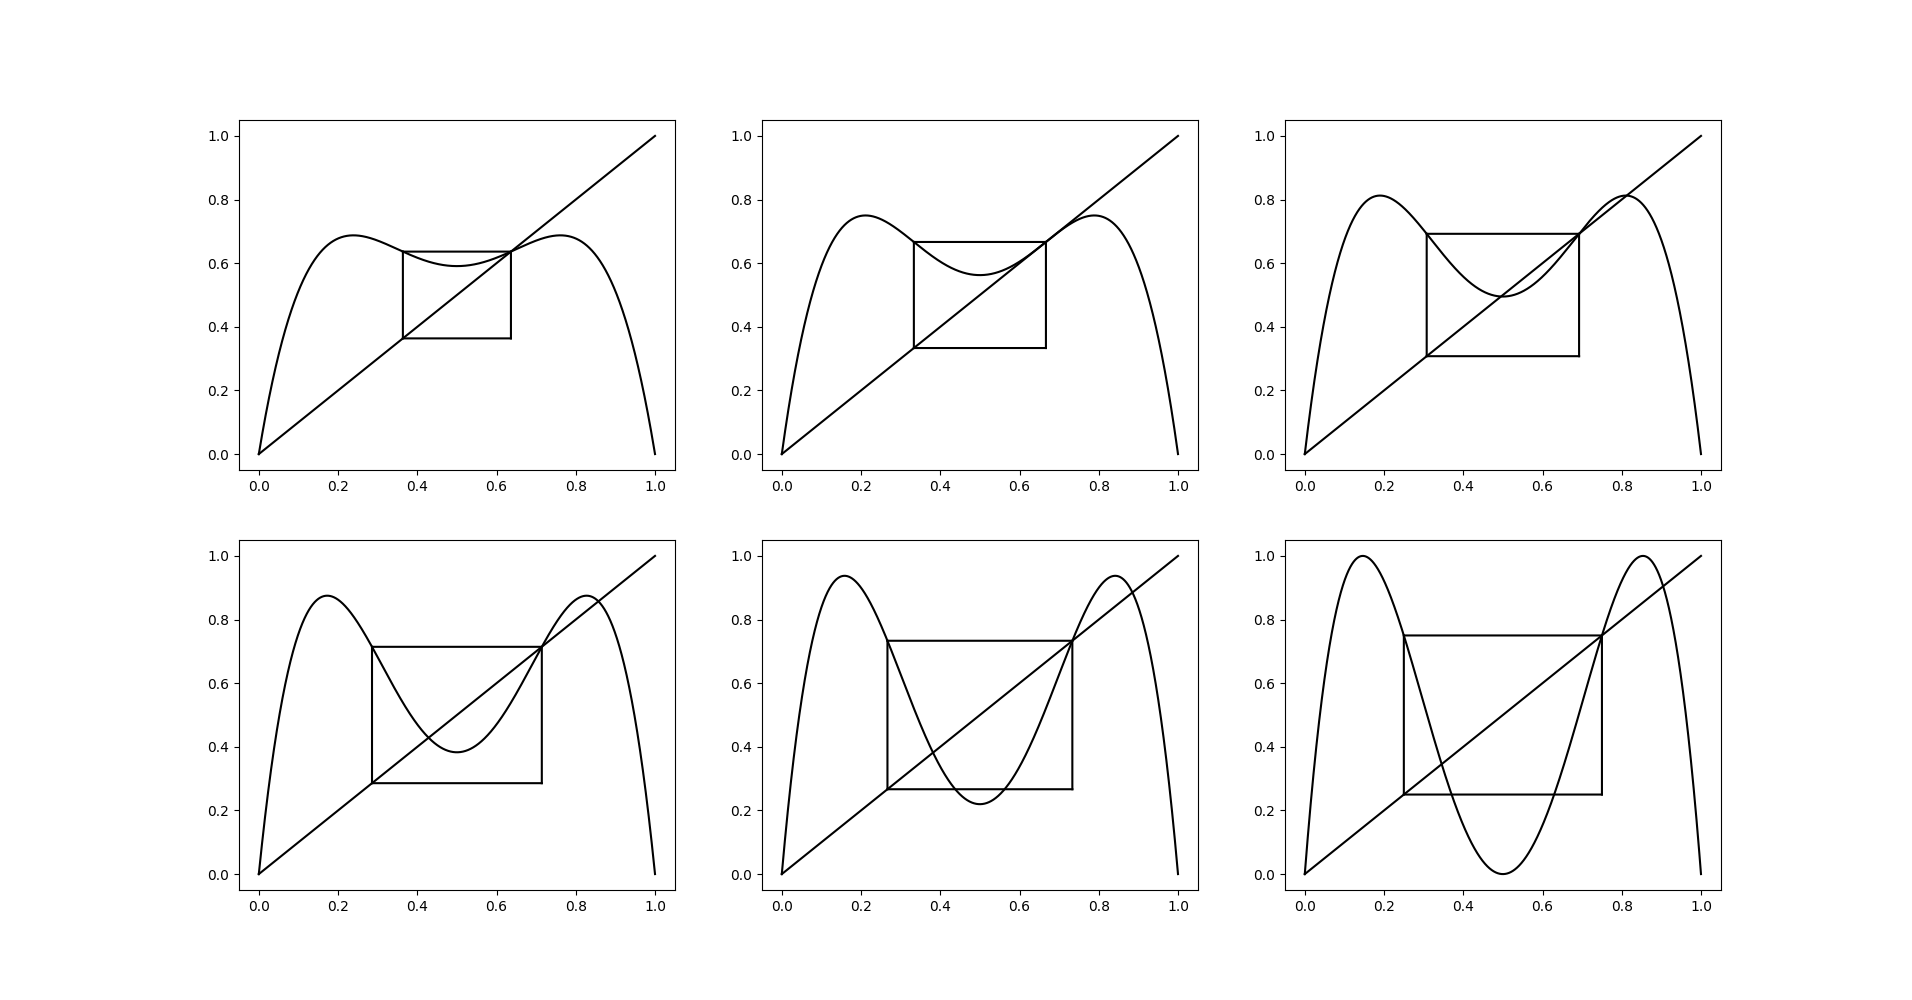
\includegraphics[scale=0.3]{images/h^2-and-boxes.png}
\end{center}

Restringindo o gráfico de $h^2$ restrito ao quadrado e rotacionando em $2 \pi$, vemos que ele se assemelha ao gráfico da própria $h$ no intervalo $[0, 1]$ para algum valor de $\mu$. Vamos deixar essa ideia mais precisa através do operador de renormalização, que nos permite analisar a segunda iterada de uma função na mesma escala que a original.

Se $\mu > 2$, considere a função $L: [p_\mu', p_\mu] \to [0, 1]$ dada por
$$L(x) = \frac{x - p_\mu}{p_\mu' - p_\mu}.$$
Observe que $L(p_\mu) = 0$ e $L(p_\mu') = 1$. Desse modo, definimos a renormalização de $h$ como a função $Rh: [0, 1] \to [0, 1]$ dada por $Rh(x) = L \circ h^2 \circ L^{-1}(x)$.

Observe que um ponto fixo de $Rh$ está unicamente relacionado com um ponto periódico de $h$ de período $2$. Além disso, o gráfico de $Rh$ não está contido em $[0, 1]$ para algum $\mu < 4$. Desse modo, podemos fazer uma análise análoga para concluir que $Rh$ passa por uma bifurcação com duplicação de período. 

\begin{center}
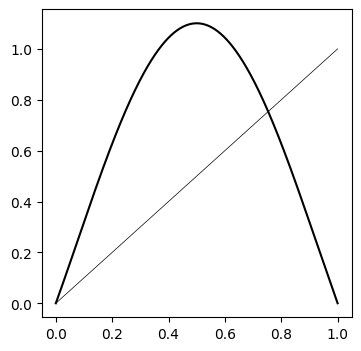
\includegraphics[scale=0.3]{images/renormalization.png}
\end{center}

Portanto, esperamos que $Rh$ sofra uma bifurcação com duplicação de período conforme o parâmetro cresce e, de maneira análoga, fazemos uma renormalização para concluir que $h^2$ sofre uma bifurcação com duplicação de período. Continuando esse processo, temos uma sucessão de bifurcações com duplicação de período na família quadrática.

O computador nos permite observar esse fato experimentalmente. Para isso, vamos computar o digrama de órbita do ponto crítico da família quadrática para $\mu > 2$. Nesse diagrama, veremos o comportamento assintótico de órbita de $\frac{1}{2}$ em função do parâmetro. Como veremos no Teorema de Singer, se $h$ possui uma órbita periódica, então ela atrai o ponto crítico. Escolhemos $2000$ valores de $\mu$ igualmente espaçados em $[2, 4]$ e, para cada valor, calculamos as primeiras $500$ iterações da órbita de $\frac{1}{2}$ e plotamos as últimas $400$.

Na figura, vemos alguns fatos que já estudamos. Para $\mu \in [2, 3]$, as órbitas são atraídas para o ponto fixo $p_\mu$ e, quando $\mu$ passa de $3$, nasce uma órbita periódica de período $2$. 

\begin{center}
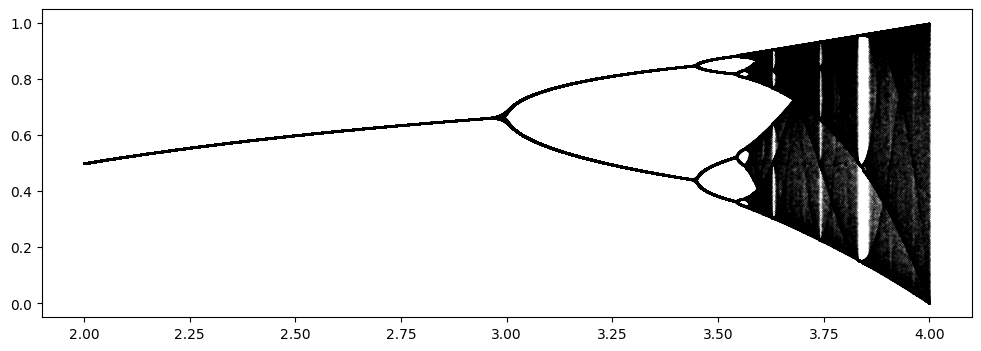
\includegraphics[scale=0.3]{images/period-doubling.png}
\end{center}

\begin{center}
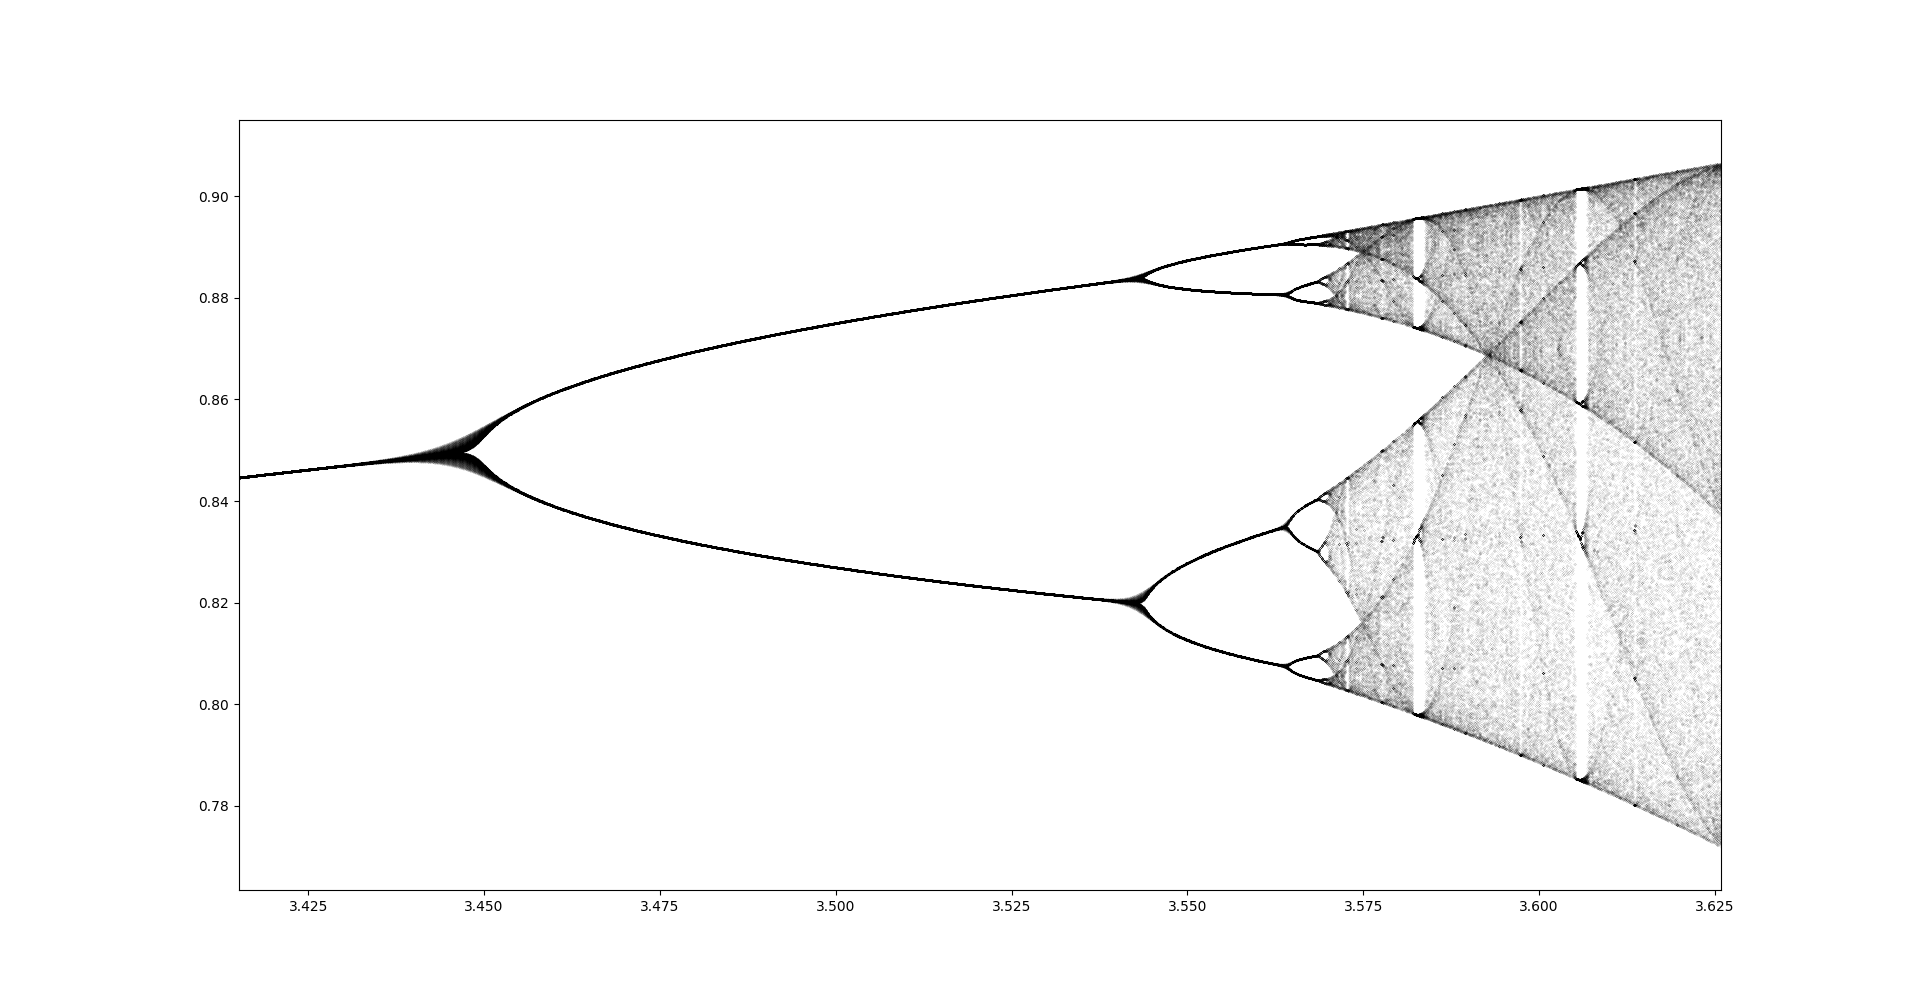
\includegraphics[scale=0.3]{images/period-doubling1.png}
\end{center}